%version of 05-27-19

\chapter{THE ART OF COUNTING, WITH APPLICATIONS: \\
Combinatorics, Probability, and Statistics}
\label{ch:prob-stat}
\label{ch:combinatorics}

We have named this chapter in honor of the great German mathematician
Gottfried Leibniz, \index{Leibniz (Leibnitz), Gottfried Wilhelm} whose
1666 doctoral thesis, ``{\it Dissertatio de Arte Combinatoria}''
\cite{Leibnitz}, gave us the now-common phrase, ``the art of
counting.''  The word ``counting'' in this context must be understood
much more broadly than in the vernacular: In days past, the phrase
encompassed much of the field known nowadays as {\it
  combinatorics}. \index{combinatorics}

Our study of the field of combinatorics can be viewed in certain ways
as a return to Chapter~\ref{ch:sets-BA-logic}'s study of
sets---especially finite sets.  Indeed, the first topics we cover in
this chapter involve looking at sets ``from the inside'', to determine
how many elements (of a certain type) the set contains
(Section~\ref{sec:counting}).

The tools we develop for determinng the cardinalities of finite sets
give us access to the important (and fun!)~field known as {\em
  combinatorial probability} \index{combinatorial probability}
(Section~\ref{sec:prob-stat}).  Have you ever wondered why the game of
($5$-card) poker values three-of-a-kind more highly than two-pair, or
why the designers of roulette tables added two (green) extra slots to
the red and black slots of the wheel?  By the end of
Section~\ref{sec:prob-stat}, you will have the wherewithal to answer
myriad such questions.

 **HERE

Just as engineering can be viewed as the ``applied'' sibling of
science, {\it statistics} can be viewed as the ``applied'' sibling of
probability.  (Section~\ref{sec:statistics})


While
Leibniz is best known (at least among mathematicians) for his
never-to-be-settled dispute with Isaac Newton \index{Newton, Isaac}
over prior discovery of the calculus, Leibniz's life was in fact
dedicated to a broad range of topics in mathematics and philosophy.
The title of his 1666 doctoral thesis, ``{\it Dissertatio de Arte
  Combinatoria}'' \cite{Leibnitz}, gave us the now-common phrase,
``the art of counting.''  The 

 was devoted to the
underpinnings of the field we know now as {\it combinatorics}; indeed, 
focused on ``the art oc counting''
({\it Arte Combinatoria}) 



\section{The Fundamentals of Counting}
\label{sec:counting}


\subsection{Binary Strings and Power Sets}

\begin{prop}
\label{thm:b-ary strings}
For every integer $b > 1$, there are $b^n$ $b$-ary strings of length
$n$.
\end{prop}

\begin{proof}
The asserted numeration follows most simply by noting that there are
always $b$ times as many $b$-ary strings of length $n$ as there are of
length $n-1$.  This is because we can form the set of $b$-ary strings
of length $n$ as follows.  Take the set $A_{n-1}$ of $b$-ary strings
of length $n-1$, and make $b$ copies of it, call them $A^{(0)}_{n-1},
A^{(1)}_{n-1}, \ldots, A^{(b-1)}_{n-1}$.  Now, append $0$ to every
string in $A^{(0)}_{n-1}$, append $1$ to every string in
$A^{(1)}_{n-1}$, \ldots, append $\bar{b} = b-1$ to every string in
$A^{(b-1)}_{n-1}$.  The thus-amended sets $A^{(i)}_{n-1}$ are mutually
disjoint (because of the terminal letters of their respective
strings), and they collectively contain all $b$-ary strings of length
$n$.  \qed
\end{proof}

\medskip

\addcontentsline{toc}{subsubsection}{-- A fun result: $n$-element sets
  have $2^n$ subsets}

\begin{prop}
\label{thm:power-sets}
The power set $\p(S)$ of a finite set $S$ contain $2^{|S|}$ elements.
\end{prop}

\begin{proof}
Let us begin by taking an arbitrary finite set $S$---say of $n$
elements---and laying its elements out in a line.  We thereby
establish a correspondence between $S$'s elements and positive
integers: there is the first element, which we associate with the
integer $1$, the second element, which we associate with the integer
$2$, and so on, until the last element along the line gets associated
with the integer $n$.

Next, let's note that we can specify any subset $S'$ of $S$ by
specifying a length-$n$ {\em binary (i.e., base-$2$) string}, i.e., a
string of $0$'s and $1$'s.  The translation is as follows.  If an
element $s$ of $S$ appears in the subset $S'$, then we look at the
integer we have associated with $s$ (via our linearization of $S$),
and we set the corresponding bit-position of our binary string to $1$;
otherwise, we set this bit-position to $0$.  In this way, we get a
distinct subset of $S$ for each distinct binary string, and a distinct
binary string for each distinct subset of $S$.

Let us pause to illustrate our correspondence between sets and strings
by focussing on the set $S = \{a,b,c\}$.  Just to make life more
interesting, let us lay $S$'s elements out in the order $b,a,c$, so
that $b$ has associated integer $1$, $a$ has associated integer $2$,
and $c$ has associated integer $3$.  We depict the elements of $\p(S)$
and the corresponding binary strings in the following table.
\begin{center}
\fbox{
\begin{tabular}{c|c|c}
Binary string & Set of integers & Subset of $S$ \\
\hline
$000$ & $\emptyset$ & $\emptyset$ \\
$001$ & $\{3\}$     & $\{c\}$ \\
$010$ & $\{2\}$     & $\{a\}$ \\
$011$ & $\{2,3\}$   & $\{a,c\}$ \\
$100$ & $\{1\}$     & $\{b\}$ \\
$101$ & $\{1,3\}$   & $\{b,c\}$ \\
$110$ & $\{1,2\}$   & $\{a,b\}$ \\
$111$ & $\{1,2,3\}$ & $\{a,b,c\} =S$
\end{tabular}
}
\end{center}

Back to the Proposition: We have verified the following: {\em The
  number of length-$n$ binary strings is the same as the number of
  elements in the power set of $S$!}  The desired numeration thus
follows by the ($b=2$) instance of Proposition~\ref{thm:b-ary
  strings}.  \qed
\end{proof}

\begin{quote}
The binary string that we have constructed to represent each set of
integers $N \subseteq \{0, 1, \ldots, n-1\}$ is called the {\it
(length-$n$) characteristic vector}\index{characteristic vector}
{\it of the set} $N$.  Of course, the finite set $N$ has
characteristic vectors of all finite lengths.  Generalizing this idea,
{\em every} set of integers $N \subseteq \N$, whether finite or
infinite, has an {\em infinite} characteristic vector, which is formed
in precisely the same way as are finite characteristic vectors, but
now using the set $\N$ as the base set.
\end{quote}


\ignore{****************8
\section{The Elements of Probability}
\label{ch:prob-stat}

 within discrete frameworks, including introducing
discrete probability/likelihood as a ratio:
\[ 
\frac{\mbox{number of targeted events}}{\mbox{number of possible events}}
\]


Elements of probability theory and statistics infuse every area of
computing.  The practicality of many algorithms that are
experientially the most efficient for their target tasks depend on the
{\em distribution} of inputs in ``real" situations.  Design
methodologies for crucial complex circuits must acknowledge the {\em
  mean times to failure} of the critical components of the circuits.
Sophisticated searching algorithms must take into account the relative
{\em likelihoods} of finding one's goal in the various optional search
directions.  Analyzing and understanding large corpora of data
requires a variety of methodologies that build on the concepts of {\em
  clustering} and/or {\em decomposition}.

A student needs at least an introduction to the foundations of
probability and statistics to even understand, all the moreso to
master, the terms highlighted in the preceding paragraph.  We outline
many of the key concepts that a student must be exposed to in the
following subsections.
**********}

{\Denis I don not know where to put the following subsection...}

\subsection{The Basic Elements of Combinatorial Probability}

Perhaps the easiest and most engaging way to introduce ``probability
via counting" is by calculating the comparative likelihoods of various
deals in $5$-card poker and of various rolls of a pair of dice.  The
arithmetic required for this discussion is elementary and the
``application" to gambling of interest even to non-gamblers: ``Why is
such a deal in poker (say, a straight) worth more than another (say,
three of a kind)?"  One can also introduce in this setting concepts
such as randomness, bias, etc., that are so important in the design of
experiments and the analysis of their outcomes.


\ignore{************
\section{Toward a Basic Understanding of Statistics}

Most students whose interest tend to the empirical will likely ``do"
statistics with the aid of apps, rather than by explicitly writing
programs that perform the required calculations.  That said, all
students should understand the crucial notion of {\em random variable}
and should be conversant with the most common statistical
distributions.  ``Conversant" in this context should include complete
understandings of the (low-numbered) moments of {\em at least} the
{\em uniform} and {\em exponential} distributions.  They should know
how to compute, say, the means and variances of various distributions
— and, most importantly, they should {\em understand} the sense in
which the variance of a distribution give {\em important} information
that is not available from the mean.  All of this is prerequisite to
rigor in experimentation.

\subsubsection{The Elements of Empirical Reasoning}

Empirical reasoning does not convey the certitude that formal
reasoning does.  Students should understand how to craft experiments
in a way that collects the ``right'' data.  The should then be
able---perhaps just with statistical packages---to interpret the
results they collect and to understand what conclusions are
justifiable.  {\em It is essential that all students understand the                  
  distinction between {\em positive correlation} and {\em causation}!}
(Most of the public would seem to flunk that test.)

In order to satisfy the preceding demands, students should understand
enough about statistics---including definitions and meanings related
to distributions and their moments---to understand what conclusions
can be made based on experimental results, and to understand how to
describe conclusions in a way that is supported by the statistics.
***********}

\section{Introduction to Probability}
\label{sec:prob-stat}


Elements of probability theory and statistics infuse every area of
computing.  The practicality of many algorithms that are
experientially the most efficient for their target tasks depend on the
{\em distribution} of inputs in ``real" situations.  Design
methodologies for crucial complex circuits must acknowledge the {\em
  mean times to failure} of the critical components of the circuits.
Sophisticated searching algorithms must take into account the relative
{\em likelihoods} of finding one's goal in the various optional search
directions.  Analyzing and understanding large corpora of data
requires a variety of methodologies that build on the concepts of {\em
  clustering} and/or {\em decomposition}.

A student needs at least an introduction to the foundations of
probability and statistics to even understand, all the moreso to
master, the terms highlighted in the preceding paragraph.  We outline
many of the key concepts that a student must be exposed to in the
following subsections.

{\Denis Here we may be more precise about the content:  first, the probabilities are built upon combinatoric rules, another interesting point is to distinguish between probability and statistics...}


\section{Elements of Combinatorics}

Add here a brief introduction,
in particular, I think we should add a link with what we have already presented many concepts pigeon holes, 
Pascal's triangle, binomial coefficients, etc..


\subsection{Counting}

The idea of counting by the way of using set theory is to establish analogies between an \textit{event}
and another (usually more abstract) event that can be studied more easily. 
Once such correspondences have been identified, we can use operations on the cardinality of the sets
for determining a \textit{number}.
The simplest situation is when the sets have one to one correspondence (thus, their cardinals are the same), or
by using operators,
{\Denis  make a link here in the chapter Arithmetic and Sets}
the most common ones are additive and multiplicative operators.

{\Denis In the original text, the multiplicative rule was presented by means of strings, which is interesting. We should choose what is the most relevant presentation. I like the way to put rules and then, to use the rules in the proofs, but I am open... I added the property of the number of }

\begin{itemize}
\item
Bijection rule:

Two sets in bijection have the same cardinality.
\item
Additive rule (also called inclusion/exclusion):

This operation (and subtraction) is obtained by unions of sets, as we described in chapter~\ref{put ref here}.
When two sets $A$ and $B$ have no common elements, then

$|A \cup B| = |A| + |B|$

if they intersect, then $|A \cup B| = |A| + |B| - |A \cap B|$.
\begin{figure}[h]
\begin{center}
        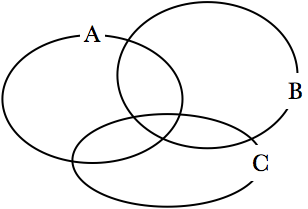
\includegraphics[scale=0.4]{FiguresMaths/3sets}
        \caption{Three sets $A,B$ and $C$.}
        \label{fig:unionSetsInit}
\end{center}
\end{figure}

Fig.~\ref{fig:unionSets} gives a clear way to extend the previous expression to more than two sets (three in the figure).
\begin{figure}[h]
\begin{center}
        
\includegraphics[scale=0.4]{FiguresMaths/RuleAdditive}
        \hspace{1cm}
        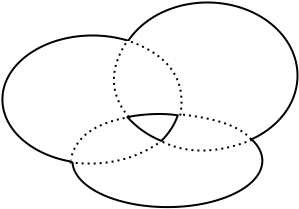
\includegraphics[scale=0.4]{FiguresMaths/RuleAdditive2}
        \caption{Union of sets $A,B$ and $C$ (left) and their intersections (right).}
        \label{fig:unionSets}
\end{center}
\end{figure}

More formally, we have to substract the two-by-two intersections of $A$, $B$ and $C$ (which each counts for $2$), 
but then, we must add the whole intersection, which counts for $3$. 
$|A \cup B \cup C| = |A| + |B| + |C| - |A \cap B| - |A \cap C| - |B \cap C| + |A \cap B \cap C|$.

%Notice here that if the sets are all disjoint, then, the cardinal of the union is the sum of the cardinal of each set.

\item
Multiplicative rule:

This operation corresponds to cartesian products of sets.
They represent all the possibilities to combine an element of the first set $A$ with an element of $B$
(see Fig.~\ref{fig:cartesianproduct} for an illustration). 
\begin{figure}[h]
\begin{center}
        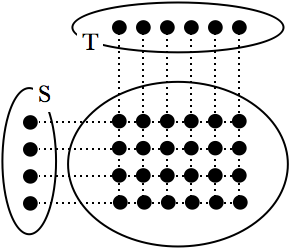
\includegraphics[scale=0.4]{FiguresMaths/cartesianProduct}
        \caption{Cartesian product of the two sets $A$ and $B$.}
        \label{fig:cartesianproduct}
\end{center}
\end{figure}

$|A \times B| = |A|.|B|$

Such a multiplicative operation can easily be extended to more than 2 dimensions: 

$|A \times B \times C| = |A|.|B|.|C|$.

In particular, $|A \times A ... \times A| = |A|^p$.
If $A$ is the set of $n$ elements $a_i$,
the cartesian product is composed of \textit{words} of length $p$.
\end{itemize}


\subsection{Preliminary on permutations}

Let consider an ordered set of $n$ items. 
As a simple abstraction, let say that the items coincide with their index.

A permutation is a $n$-tuple $(x_1,x_2, \ldots , x_n)$ where each number appears only once. 
For instance, 
$(3,2,1,4)$ is a permutation of the four first integers. 
The purpose of the following proposition is to count the number of permutations.
\bigskip

\begin{prop}
The number of permutations of the first $n$ integers is equal to $n!$
\end{prop}

\begin{proof}
The proof is by recurrence and the proposition is obviously verified for $n=1$.

Let assume it is true at order $n$ and consider a permutation $(x_1, \ldots , x_n, x_{n+1})$ of order $(n+1)$.
The element in position $k$ ($1 \leq k \leq n+1$) can take any of the $n+1$ different values
and the remaining positions $(x_1, \ldots , x_{k-1}, x_{k+1}, \ldots, x_{n+1})$
are all the permutations of order $n$ with the remaining integers.
Thus, the number of permutations is equal to $\sum_{k=1}^{n+1} n! = (n+1)!$
\end{proof}


%%%%%%%%%%%%%%%%%%%%%%%

\subsection{Combinations}

The combinations are strongly linked with the binomial coefficients that are presented 
in Section~\ref{sec:binomial-coeff}.
We analyzed some properties in Section~\ref{sec:binomial-coeff+Pascal}.

The expression of the binomial coefficient is:
\[ {n \choose k} \ = \ \frac{n(n-1)\ldots(n-k)}{k!} \]
We proved this expression by recurrence, here is a combinatorial argument:

The number of sequences of $k$ elements among $n$ is equal to n(n-1)\ldots(n-k)

The number of orderings of a set of $k$ elements is $k!$

The number of ways to choose $k$ over $n$ is the ratio of both previous factors.

\medskip

In the cartesian product  $A \times A ... \times A$, there are words with multiple $a_i$.
For instance, considering $A=\{ 1,2,3 \}$, the element $(3,2,3,1)$ of $A^4$ contains twice the element $a_3=3$ 
or $(1,2,1,1)$ contains three times $a_1=1$. 
A natural question is to study what happens if we want only the words with different components?


\subsection{Derangements}

Derangements of a set $A$ is a bijection without \textit{fixed points}.
This means that we donot allow an element to be associated to itself
or (using a more formal vocabulary), there is no cycle of length 1 in the strings of $A^n$
($n$ is the cardinal of $A$).

Let denote by $d(n)$ the number of derangements.
\medskip

Consider for instance the set $A = \{1,2,3 \}$, there are two derangements, namely
($1 \rightarrow 2$, $2 \rightarrow 3$, $3 \rightarrow 1$)
and 
($1 \rightarrow 3$, $2 \rightarrow 1$, $3 \rightarrow 2$).
\medskip

$d(1) = 0$ and $d(2) = 1$

$d(n) = (n-1) (d(n-1) + d(n-2))$

$d(n) = (-1)^n + n d(n-1)$
\bigskip

By the principle inclusion/exclusion, we show that the complexity is roughly of order $n!$

As the number of objects increases, the probability that none appears in its correct position approaches
$p=lim_{n \rightarrow \infty}\frac{d(n)}{n!}=\frac{1}{e}$. 

{\Denis Interesting: to be detailed in more details...}


\section{The Elements of Combinatorial Probability}

Perhaps the easiest and most engaging way to introduce ``probability
via counting" is by calculating the comparative likelihoods of various
deals in $5$-card poker and of various rolls of a pair of dice.  The
arithmetic required for this discussion is elementary and the
``application" to gambling of interest even to non-gamblers: ``Why is
such a deal in poker (say, a straight) worth more than another (say,
three-of-a-kind)?"  One can also introduce in this setting concepts
such as randomness, bias, etc., that are so important in the design of
experiments and the analysis of their outcomes.

Let recall that games can be characterized by pure gambling -- random games (dices and wheels), 
mental games (board games like chess or GO)
 {\Denis I don't know the english term for the games that challenge the mind...} 
and mixed ones (Backgammon, Bridge or Poker).
\medskip

Introducing discrete probability/likelihood as a ratio:
\[ 
\frac{\mbox{number of targeted events}}{\mbox{number of possible events}}
\]

We have several immediate consequences:

First, since the number of targeted events is lower than the number of all possible events,
the probability is lower than $1$. 

It is also positive, and a probability $0$ corresponds to the probability of an empty event.

An event is as probable as its probability is close to 1.

Using the additive rule, the probability of two distinct series of events is equal to the sum of the probabilities
of both events. 
In particular, the probability of two complementary events is equal to 1 (obtained by $p + (1-p)$).


\subsection{Illustration: Playing Poker}

Let us consider a usual deck of 52 cards composed of $n=13$ figures:

\textit{(2,3,4,5,6,7,8,9,10,Jack,Queen,King,Ace)} 

on the 4 colors \textit{(club, diamond, heart and spades)}.

The total number of possible \textit{hands} (i.e. set of the 5 cards owns by each player) is 
${32 \choose 5} = \frac{52!}{5! 47!} = 2 598 960$, this is a huge number of possibilities that makes the Poker game an interesting one.

The patterns that characterize the game in a hand can be classified by their number of occurrences.
Let survey briefly the principal ones.

\begin{itemize}
\item
There are only 4 different ways to form a royal flush (i.e. the 5 cards  \textit{(10,J,Q,K,Ace)} of the same color). 
Thus, the probability of getting such an hand is equal to $\frac{4}{2 598 960}$ that is one over $649740$, which is equal to $0.000154$.
\item
Now, let us calculate the number of hands within a straight flush, excluding the royal flush.

The reasoning is similar as for the royal flush, taking into account that there are $9$ possible series of $5$ consecutive cards
(from \textit{(Ace,2,3,4,5)}, \textit{(2,3,4,5,6)}, and so on --- shifted progressively --- to \textit{(9,10,J,Q,K)}).

Thus, as the flush requires to have the same color, there are $9 \times 4 = 36$ such hands. 
\item
Four-of-a-kind.

There are $13$ possible cards. There is a remaining card left that is any one among the 48 remaining ones.
Indeed, according to the multiplicative principle, it remains ${12 \choose 1}$ in each of the $4$ colors. 
Thus, $13 \times 48 = 624$, which corresponds to the probability $0.00256$.
\item
Three-of-a-kind and Full Houses.

The analysis of the first of these two patterns follows the same logic as for the Four-of-a-kind.
Again, there are as many possibilities of the $3$ base cards of the pattern than the number of cards in a color ($13$)
with only $3$ colors among the 4: ${4 \choose 3}$.
The two remaining cards should be different from the kind (and different from each other), 
thus, their number is to select $2$ among the $12$ remaining ones,
each one can take any colors (their number is $4^2$).
The final expression is:

$13.{4 \choose 3}.{12 \choose 2}.4^2 = 858$

For getting a Full House, the enumeration is close to the previous one, but there is a slight difference 
on the two remaining cards,
which here should by a pair (two of the same kind, that is only $1$ card among the $12$, 
this card can take any of the four colors),
thus:

$13.{4 \choose 3}.{12 \choose 1}.4 = 156$
\end{itemize}


\subsection{Monthy Hall}

The following example is a true story which shows that reasoning with probability is not easy (and not natural at all). 
It comes from a popular TV-show in the 70th and 80th. 
The show, named \textit{Let's make a deal}, was presented by  Monthy Hall.
A jackpot were hidden behind one of three doors. 
The game consisted to ask someone to guess the right door (where is located the jackpot)
for wining the jackpot.
Once the choice is done, Monthy Hall opened one of the two other doors (obviously, one without the jack pot)
and ask the candidate whether she wants to change her choice or to keep her initial choice.

Choosing one door among three corresponds to a probability to win equal to one third.
Most people think it is not worse if they change their choice.
However, as proposed by Marylin von Savant, it is better to change. 
Here is her reasoning
(it is illustrated in Fig.~\ref{fig:MonthyHall}):
\begin{figure}[h]
\begin{center}
        \includegraphics[scale=0.5]{FiguresMaths/MonthyHallInitial}
%                \includegraphics[scale=0.5]{FiguresProba/MonthyHallInitial}
        \caption{The three doors of \textit{let's make a deal}.}
        \label{fig:MonthyHall}
\end{center}
\end{figure}

We proceed case by case as follows.
\begin{itemize}
\item
If we select the right door at the beginning, keeping the same choice leads to the same probability 
as the first choice, that is one third.
\item
If we select a wrong door (which will arrive with a probability of two third), we win the jackpot if we change this choice.
%because now the choice in among two cases. 
\begin{figure}[h]
\begin{center}
        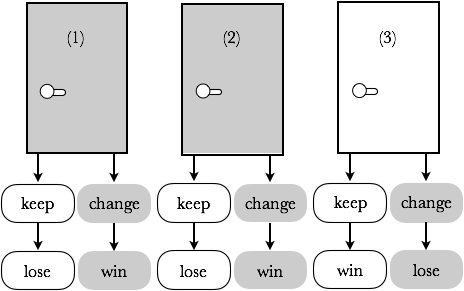
\includegraphics[scale=0.4]{FiguresMaths/MonthyHall}
%                \includegraphics[scale=0.4]{FiguresProba/Monthy}
        \caption{Suppose the jackpot is behind door (3). 
        If we select it, we lose if we change the initial choice.
        However, it is better to change if we select one of both other doors (1) or (2).}
        \label{fig:MonthyHall}
\end{center}
\end{figure}
\end{itemize}

Remark: this result does not seem to be very natural. Ask your neighbor about this experience
and she will probably tell you that changing does not matter.
It was a great polemic at the time of the show.


\subsection{The anniversary Paradox}

We present here another application of the rules of enumeration to calculate the probabilities~\cite{DumasTrystram}.
It shows in particular that it is sometimes easier to calculate the probability that an event does not occur than the direct
event. 

As teachers, we are commonly asking the students in the Maths class if there are some of them who are born the same day.
As the class is about 30 students, the answer is usually \textit{yes}. 
Is it by chance?
Then, we ask how many students do we need to obtain a probability at least one half (50\%) to have the anniversary the same day.
We develop the method below.
\bigskip

Let consider a common year with 365 days. 
A first and obvious remark is that it is sufficient to have 366 people since the worst case is obtained when the anniversary 
of the first 365 people is in a different day. This is another illustration of the pigeon hole principle. 
Can we expect to have $366/2 = 183$ people to obtain a probability of $50\%$?
\bigskip

Let us analyze the situation in more detail and consider the dual problem of determining the probability 
not to have the anniversary the same day (the initial probability is 1 minus this one...). 
Denote $\pi(n)$ this probability.

Consider a class of $n$ student and take one of them randomly ($n \leq 365$).
She or he can have her anniversary any of the 365 days. 
and similarly for the $n-1$ remaining ones. 
Thus, the number of all possible cases is $365^n$. 
Now, we focus on the first student: there are 365 ways to choose her birth date.
As we are looking for different dates, there is only 364 choices for the second student and so on until $365-(n-1)$ 
for the last one.
Thus, the number of positive choices is equal to $365 \times 364 \times \ldots \times (366-n) = \frac{365!}{(365-n)!}$.

\[ 
\pi(n) = \frac{\mbox{number of positive choices}}{\mbox{number of possible choices}} = \frac{365!}{ (365-n)!  \times 365^n}
\]

If we come back to the probability to have the anniversary the same day (which is equal to $1-\pi(n)$),
we obtain $0.5073$ for $n=23$: in other words, we have slightly more than $50\%$ chances to have two students born 
the same day 
in a class with 23 students.
For our classes with $30$ students, the probability grows up to $0.70632$. 

{\Denis Another interesting variant is to determine the probability of a student to be born the same day as me. This may be a good exercice. Quite easy.}


\subsection{Sum of three dice}

If chess is a pure thinking game, there are pure random games
(and some intermediate games which mixed smart strategies and randomness like Backgammon).
In particular, the very old games that are based on rolling three 6-sided dice games,
with some variants that still exist today (for instance the $421$ game).

The goal is to roll the three dice in order to obtain a certain value of the sum.
Assuming an equiprobability on each face of the dice, we can analyze the game by an enumeration of all
the possible results. 

%Let us first discuss the enumeration
%and then, let us extend the analysis where the dices are separate ones.
\bigskip

The enumeration leads to $56$ configurations, and this result can be obtained in two different ways
as we are developing below.
\begin{itemize}
\item 
The first manner is to enumerate one after the other all the numbers of ways to obtain a possible value of the sum.
Starting at $3$ which is the smallest possible value (since the dice sides are each numbered from $1$) to $18$
when the three dice have a $6$.

\begin{tabular}{|c|c|c|c|c|c|c|}
\hline
 & & & & & & sum\\
\hline
111 & & & & & & 3\\
112 & & & & & & 4\\
113 & 122 & & & & & 5 \\
114 & 123 & 222 & & & & 6 \\
115 & 124 & 133 & 223 & & & 7\\
116 & 125 & 134 &  224 & 233 & & 8\\
126 & 135 & 144 & 225 & 234 & 333 & 9\\
136 &  226 & 145 & 244 & 235 & 334 & 10\\
146 & 236 & 155 & 245 & 335 & 344 & 11\\
156 & 246 & 336 & 255 & 345 & 444 & 12\\
166 & 256 & 346 & 445 & & & 13\\
266 & 356 & 446 & 455 & & & 14\\
366 & 456 & 555 & & & & 15\\
466 & 556 & & & & & 16\\
566 & & & & & & 17\\
666 & & & & & & 18\\
\hline
\end{tabular}
\smallskip

From the previous table, we can easily deduce the probability to obtain a sum equal to 6
by applying the definition: $p(6) = \frac{4}{56}=0.071\ldots$
\item 
The other way to enumerate is based on 
a partition of the configuration sets of the three dice, namely,
the set where the three dice have the same value, the set where the is a common value in two dice
and the set where the dice are all different. 
In this last case, the enumeration is simplified if we consider that the dice values are all consecutive,
if two of these values are contiguous and if there are all non contiguous.

More precisely, there are obviously $6$ ways to obtain a sum where the dice are all the same (one per side).
There are $6 \times 5 = 30$ ways to make a sum where two dice are the same. 
And there are $20$ ways for a sum with three different values. 
Thus, a total of $56$ like before.
\end{itemize}

\bigskip
Let us study now a little variant of the enumeration of the configurations
where the value of a die matters.
In the previous table, obtaining a sum of $6$ was done by three different configurations:
\begin{enumerate}
\item one die of each value $1$, $2$, $3$
\item two dice of $1$ and one $4$
\item three dice $2$
\end{enumerate}

A sum of three dice equal to $6$ (and symmetrically $15$) can be obtained by $10$ different manners as follows
(each column is a roll):
\medskip

\begin{tabular}{|l|c|c|c|c|c|c|c|c|c|c|}
\hline
First die & 1 & 1 & 4 & 1 & 1 & 2 & 2 & 3 & 3 & 2   \\

Second die & 1 & 4 & 1 & 2 & 3 & 3 & 1 & 1 & 2 & 2   \\

Third die & 4 & 1 & 1 & 3 & 2 & 1 & 3 & 2 & 1 & 2  \\
\hline
\end{tabular}

\medskip

We let the reader verify the following table that gives this number for each possible sum.
The number of all possible configurations is $6^3=216$ and we verify easily that this number is equal to:
$2 \times (1 + 3 + 6 + 10 + 15 + 21 + 25 + 27)$.
\medskip

\begin{tabular}{|l|c|c|c|c|c|c|c|c|}
\hline
Sum & 3 and 18 & 4/17 & 5/16 & 6/15 & 7/14 & 8/13 & 9/12 & 10/11  \\
\hline
$\#$config. & 1 & 3 & 6 & 10 & 15 & 21 & 25 & 27  \\
\hline
\end{tabular}
\medskip

%{\Denis This result is amazing since the series grows like the sum of the first $n_{th}$ integers, except for the last ones which are truncated. This is probably possible to prove it!}

\subsection{Synthesis and transition}

We have developed several examples, which illustrate how to compute the probability of an event,
by means of enumeration of favorable and possible cases. 
This is still valid for examples composed of many occurrences of an event,
like rolling a die or tossing coins. 

Two kind of questions may be studied.
First, "how the probability of the occurrence of an event (like obtaining a $6$) is related to practical results?"
The second question is somehow the reverse: "If we run several times an experience of rolling dices, is it possible 
to infer the corresponding probability?".

For the first question, it is easy to see that (if the die is fair) there are as many chances to get any number as the $6$
(we say that the events are \textit{equiprobable}),
thus, in other mathematical words: $p(1)=p(2)=p(3)=p(4)=p(5)=p(6)$,
and the probability is the same for any of the six values equal to $\frac{1}{6}$.
This use of probability is common: study the probability and then, deduce the future behaviors.
The second question is the main purpose of statistics that is developed in the next section.

% discuss Probability versus Statistics...

{\Denis We have to mention the links with the two other places where we discussed Binomial coefficients, recurrences and arithmetic, in this last case, we presented a question of computing the probability of getting 25 tails over 40 trials while flipping coins...}



\section{Toward a Basic Understanding of Statistics}
\label{sec:statistics}

{\Denis I copied the two following paragraphs from the existing text (written a long time ago by you...}

Most students whose interest tend to the empirical will likely ``do"
statistics with the aid of apps, rather than by explicitly writing
programs that perform the required calculations.  That said, all
students should understand the crucial notion of {\em random variable}
and should be conversant with the most common statistical
distributions.  ``Conversant" in this context should include complete
understandings of the (low-numbered) moments of {\em at least} the
{\em uniform} and {\em exponential} distributions.  They should know
how to compute, say, the means and variances of various distributions
— and, most importantly, they should {\em understand} the sense in
which the variance of a distribution give {\em important} information
that is not available from the mean.  All of this is prerequisite to
rigor in experimentation.

\subsection{The Elements of Empirical Reasoning}

Empirical reasoning does not convey the certitude that formal
reasoning does.  Students should understand how to craft experiments
in a way that collects the ``right'' data.  The should then be
able---perhaps just with statistical packages---to interpret the
results they collect and to understand what conclusions are
justifiable.  {\em It is essential that all students understand the                  
  distinction between {\em positive correlation} and {\em causation}!}
(Most of the public would seem to flunk that test.)

In order to satisfy the preceding demands, students should understand
enough about statistics---including definitions and meanings related
to distributions and their moments---to understand what conclusions
can be made based on experimental results, and to understand how to
describe conclusions in a way that is supported by the statistics.


\subsection{An old story}

The following example reports one of the oldest statistical problem.

In his paper,
\textit{An argument for divine providence taken from the constant regularity observed in the births of both sexes}
appeared in Philosophical transactions, 1710, 
% As pointed out by Bernard Ycart, this is the first known statistical reasoning~\cite{websiteBernard}.
John Arbuthnot studied the number of births over an archive of 82 years and draw the proportions of boys and girls
in London (UK) from 1629 to 1710. 
In 1629, there was  5218 males for only 4683 females and in 1710, 7640 against 7288. 
 
The observation was systematic, and the result was surprising: there are always more male births than female births
(in the proportion of about 22 to 21 as pointed out some time later by Pierre Simon Laplace in his 
\textit{Essai philosophique sur les probabilités} in 1814). 
Notice that it is still true today, and the reason has not yet been clearly identified...

Here the reasoning done by Arbuthnot:
if the births are random, then the probability to have more boys than girls should be equal to 
$p=(\frac{1}{2})^{n}$ for $n$ years of observation.
He succeeded to get the records for the last $82$ years, this means $p \rightarrow 0$.
In other word, there is a quasi null probability to have more boys than girls, which contradicts the observations. 

He looked at this problem by using an analogy with 2 face dices labelled Male and Female
(Today, we will rather talk about tossing coins). 
\medskip

The sketch of the statistical proof is as follows:

Assuming that the events (births) are independent and equiprobable,
%, and there is no difference between boys and girls.
the experience is taken over a long period (82 years), it shows that the probability to have more boys is very tiny and
tends to zero. 
Thus, the hypothesis of an even repartition is false: there are more boys than girls!
\medskip

This is an illustration of the large number law, which says that the probability can be interpreted 
as a limit of experimental measures (frequency of occurence of an event). 
\bigskip

\noindent \fbox{
\begin{minipage}{0.95\textwidth}
Probability or Statistics?

Two faces of the same thing?

Repeating a random experience more and more gives a better (accurate) value
of the relative frequency of the events.
They tend to a limit.

This is another way to look at the probability that this event occurs. 
\end{minipage}
}
\bigskip

The next section is devoted to give more details on this important law.


\subsection{The Law of Large Numbers} 
%\textit{Loi des grands nombres}}

{\Denis add ref: Jocobi Bernoulli, Ars conjectandiopus posthumum}

The former traces of the large numbers law are in a book from Jakob von Bielfeld in 1767.
Later, with the emergence of the probability theory and in particular via the swiss mathematician Jacques Bernoulli
and his nephew Nicholas who finished the work of his uncle when he died, 
the law of large numbers was given as a theorem for describing the result of performing the same experiments
 a large number of times. 
 According to this result, the average of the results obtained from a large number of experiences is close 
 to the expected value. 
For instance, a single roll of a die produces evenly one of the numbers 1 to 6.
Thus, the According to the law, if a large number of dice are rolled, the average of their values 
is likely to be close to the value $\frac{1+2+3+4+5+6}{6}=3.5$.
The precision is increasing with the number the dices are rolled. 

\bigskip

Let consider a hat containing white and black balls.
We will discuss two variants: first, the number of balls is known and second, it is not.

\begin{itemize}
\item If the proportion is known (say for instance 300 white balls and 200 black balls
(thus, $60\%$ of white and $40\%$ of black).

Clearly, there is more chance to get a white than a black.
But the Loi des grands nombres tell us a bit more: the probability to get a white is close to $60\%$
if we are drawing a ball a large number of times and putting it back in the hat.

If we are doing only one trial, the result is simply $1$ or $0$ (if I get a black or not)...
How many trials do we have to do to be sure that the probability is $60\%$?
For instance, draw ten balls, are we sure to obtain $6$ white balls? What about $100$ or $1000$?
\item If the number of balls is not known.
The experience consists in determining the probability to draw a white ball without knowing 
We proceed as before:
draw a ball, note his color and put it back in the hat, and do it again and again...
%(then, the proportion of white/black balls remains unchanged)

The loi des grands nombres will provide the answer (the limit) for an infinite number of trials.
If we want to be sure to obtain the result with a precision of $1\%$,
how many trials do we have to do to get a probability in the interval $(59.9,60.1)$?
\end{itemize}

\medskip

\noindent \fbox{
\begin{minipage}{0.95\textwidth}
In the loi des grands nombres, called also the \textit{golden theorem} (Th\'eor\`eme d'or) by Jacques Bernouilli,
large numbers refer to the convergence of the frequency of occurrence of an experience to a limit, which is the probability
that the event occurs. 

The Loi des grands nombres gives also a solution to the problem of how many trials are needed to obtain a given
precision...

\end{minipage}
}
\bigskip

I think we should conclude by the Loi normale and the gaussian distribution. 

The story is very interesting, it has been the main work of Abraham de Moivre (1667-1754), 
which studied the sum of the terms that appear in the binomial formula of Newton when the power $n$ is large.
His idea was to link with the probability of an event $n$ being the number of times this event occurs.

The binomial expression is:

$(1+x)^n = \sum_{k=0,n-1} {n \choose k} x^k = (1+x)(1+x)\ldots(1+x)$

in each of the $n$ factors $(1+x)$, choose $1$ or $x$, we obtain the coefficient of $x^k$.

\medskip

The distribution of some rows of the Pascal's triangle is given in Fig.~\ref{fig:gaussiandistribution}.

$1,10,45,120,210,252,210,120,45,10,1$ and

$1,15,105,455,1365,3003,5005,6435,6435,5005,3003,1365,455,105,15,1$.
They show a Gaussian distribution.
\begin{figure}[h]
\begin{center}
        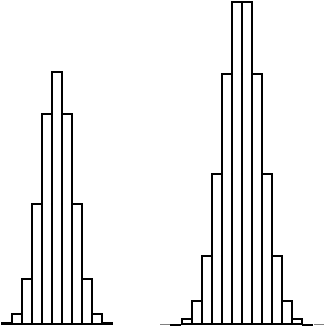
\includegraphics[scale=0.5]{FiguresMaths/ProbaGaussianDistribution}
        \caption{Distribution of the binomial coefficients in the 10th row (left) and the 15th row (right) of the Pascal's triangle.
        The scale of the right histogram is 1/20.}
        \label{fig:gaussiandistribution}
\end{center}
\end{figure}


\section{Beyond the Basics}

As students are introduced to modern topics within computing, whether
at the level of a Computing Literacy course or a post-core technical
course, they will have to master a variety of more specialized topics
that combine pieces of the elements we have discussed in this essay.
While these topics are beyond the level of generality aimed at in this
essay, some may be appropriate prerequisites to programs that have
some specialized foci.
\begin{itemize}
\item
Issues relating to {\em clustering} find application in applications as
diverse as: {\em linear-algebraic computations}, {\em data mining},
{\em design and layout of digital circuitry}.

\item
Issues building on {\em graph separation/decomposition} are
encountered when studying: {\em linear-algebraic computing}, {\em
  fault-tolerant design}, {\em load balancing}.

\item
Many issues relating to {\em fault/failure tolerance} and {\em data
  analytics} benefit from study using {\em random walks} (at least in
one dimension).

\item
Many useful ideas regarding the {\em encoding and manipulation of
  data} can be gleaned from the elements of {\em information theory}
and {\em computer arithmetic}.
\end{itemize}
The preceding list is really endless.  Hopefully readers will be
inspired by our few examples to compile a longer version that is
appropriate for their particular environments.




